\documentclass{article}
\usepackage{times}
\usepackage{tikz}
\usepackage{verbatim}
\usepackage{hyperref} 
\usepackage{graphicx}
\usepackage{natbib}
\usepackage{amsmath,amssymb}
\DeclareMathOperator*{\argmin}{arg\,min}
\DeclareMathOperator*{\sign}{sign}
\DeclareMathOperator*{\Lik}{Lik}
\DeclareMathOperator*{\Peaks}{Peaks}
\DeclareMathOperator*{\HotSpots}{HotSpots}
\newcommand{\Cost}{\text{Cost}}
\usepackage{stfloats}
\DeclareMathOperator*{\Diag}{Diag}
\DeclareMathOperator*{\TPR}{TPR}
\DeclareMathOperator*{\Segments}{Segments}
\DeclareMathOperator*{\FPR}{FPR}
\DeclareMathOperator*{\argmax}{arg\,max}
\DeclareMathOperator*{\maximize}{maximize}
\DeclareMathOperator*{\minimize}{minimize}
\newcommand{\ZZ}{\mathbb Z}
\newcommand{\NN}{\mathbb N}
\newcommand{\RR}{\mathbb R}
\definecolor{good}{HTML}{6A3D9A}
\definecolor{bad}{HTML}{1F78B4}
\definecolor{noPeaks}{HTML}{F6F4BF}
\definecolor{peakStart}{HTML}{FFAFAF}
\definecolor{peakEnd}{HTML}{FF4C4C}
\definecolor{peaks}{HTML}{A445EE}

\usepackage{icml2015}

\icmltitlerunning{PeakSeg: constrained optimal segmentation and
  supervised penalty learning for peak detection in count data}

\begin{document}

\twocolumn[
\icmltitle{PeakSeg: constrained optimal segmentation and
  supervised penalty learning for peak detection in count data}

% It is OKAY to include author information, even for blind
% submissions: the style file will automatically remove it for you
% unless you've provided the [accepted] option to the icml2015
% package.
\icmlauthor{Guillem Rigaill}{rigaill@evry.inra.fr}
\icmladdress{INRA, Evry, France}
\icmlauthor{Toby Dylan Hocking}{toby.hocking@mail.mcgill.ca}
\icmlauthor{Guillaume Bourque}{guil.bourque@mcgill.ca}
\icmladdress{McGill genome center, Montreal, Quebec, Canada}

% You may provide any keywords that you 
% find helpful for describing your paper; these are used to populate 
% the "keywords" metadata in the PDF but will not be shown in the document
\icmlkeywords{segmentation, count data, penalty functions}

\vskip 0.3in
]

\begin{abstract}
  Peak detection is a central problem in ChIP-seq data analysis, and
  current algorithms for this task are unsupervised and mostly
  effective for a single data type and pattern (e.g. H3K4me3 data with
  a sharp peak pattern). We propose PeakSeg, a new constrained maximum
  likelihood segmentation model for peak detection with an efficient
  inference algorithm: constrained dynamic programming. We investigate
  un\-super\-vised and super\-vised learning of penalties for
  the critical model selection problem. We show that the 
  super\-vised method is the first algorithm with state-of-the-art peak
  detection across all data sets in a benchmark that includes both
  sharp H3K4me3 and broad H3K36me3 patterns.
\end{abstract}

\section{Introduction}

\subsection{Unsupervised ChIP-seq peak detection}

Chromatin immunoprecipitation sequencing (ChIP-seq) is a biological
experiment for genome-wide profiling of histone modifications and
transcription factor binding sites, with many experimental and
computational steps \citep{practical}. Briefly, each experiment yields
a set of sequence reads which are aligned to a reference genome, and
then the data are interpreted by counting the number of aligned reads
at each genomic position (Figure~\ref{fig:dp-peaks-train}). In this
paper we propose a new method for peak calling these data, which is a
binary classification problem for each genomic position. The positive
class is enriched (peaks) and the negative class is background
noise. Importantly, peaks and background occur in long contiguous
segments across the genome.

\begin{figure*}[b!]
  \centering
  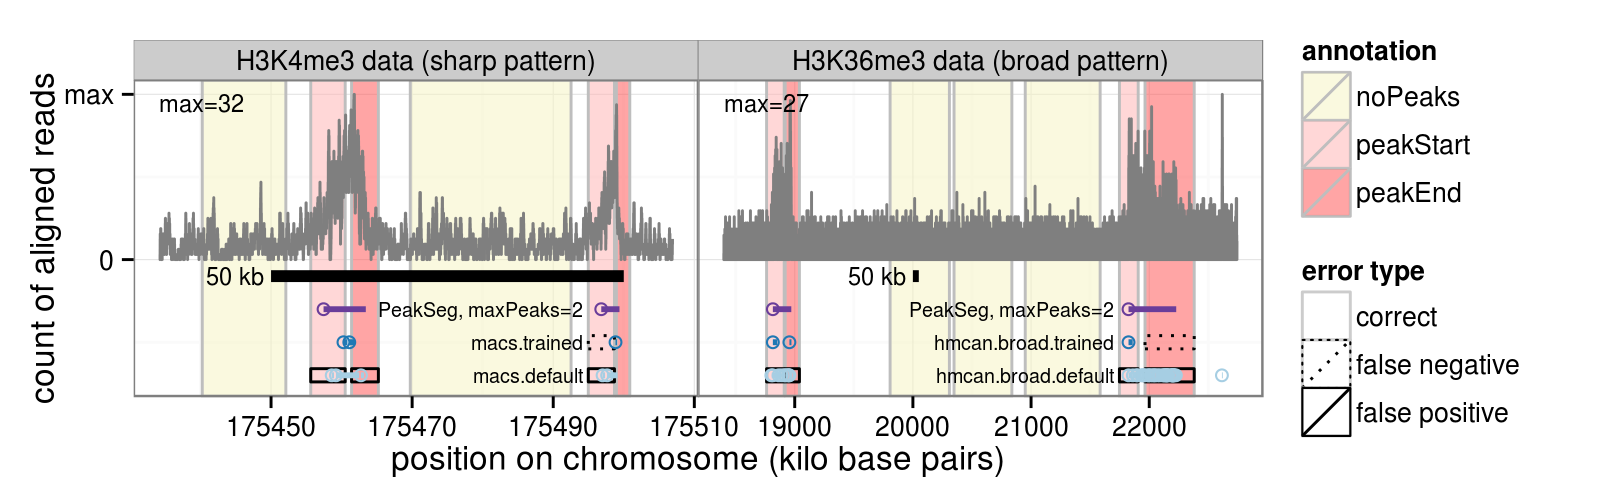
\includegraphics[width=\textwidth]{figure-dp-peaks-train}
  \vskip -0.5cm
  \caption{Different ChIP-seq data types have peaks with different
    patterns. Positions classified as peaks are drawn as line segments
    for a \textcolor{good}{good peak model} with zero errors and a
    \textcolor{bad}{bad peak model} with 7 incorrect regions. The goal
    of supervised peak detection is to learn the data set-specific
    peak pattern encoded in the annotated region labels
    (\colorbox{peakStart}{peakStart}/\colorbox{peakEnd}{peakEnd} mean
    there should be exactly 1 peak start/end somewhere in the region,
    and \colorbox{noPeaks}{noPeaks} means there should be no
    overlapping peaks).}
  \label{fig:dp-peaks-train}
\end{figure*}

More concretely, a single ChIP-seq profile on a genomic region with
$d$ base pairs can be represented as a vector $\mathbf y= \left[
  \begin{array}{ccc}
    y_1 & \cdots & y_d
  \end{array}
\right]\in\ZZ_+^d$ of counts of aligned sequence reads. A peak
detection algorithm can be described as a function $c:\ZZ_+^d
\rightarrow \{0, 1\}^d$ which returns 0 for background noise and 1 for
a peak. In contrast to the
supervised method proposed in this paper, most previous algorithms are
unsupervised since they define a peak detector $c$ using only the
profile data $\mathbf y$.


\subsection{Different ChIP-seq peak patterns}

There are several different kinds of peak patterns that have been
observed and labeled in different ChIP-seq data sets. For example,
Figure~\ref{fig:dp-peaks-train} shows H3K4me3 data with a sharp peak
pattern, and H3K36me3 data with a broad peak pattern. Current peak
detectors are unsupervised learning algorithms that are designed for
specific patterns. For example, the MACS algorithm was designed for
the sharp pattern in H3K4me3 data \citep{MACS}.

Another example is HMCan \citep{HMCan}, whose authors suggest fixed
pattern-specific mergeDistance parameters: H3K4me3 $\Rightarrow 200$,
H3K36me3 $\Rightarrow 1000$. However, these parameters may not be
optimal for any given data set.

\subsection{Supervised peak detection}

In supervised peak detection \citep{hocking2014visual}, there
are $n$ labeled samples, and each sample $i\in\{1, \dots, n\}$ has a
profile $\mathbf y_i\in\ZZ_+^d$ and a set of annotated region labels $R_i$ 
("no peak", "peak", ...).
which defines a non-convex annotation error function
\begin{equation}
  \label{eq:error}
  E[c(\mathbf y_i),  R_i] =
  \text{FP}[c(\mathbf y_i), R_i] +
  \text{FN}[c(\mathbf y_i), R_i].
\end{equation}
The annotation error counts the number of false positive (FP) and
false negative (FN) regions (Figure~\ref{fig:dp-peaks-train}), so it
takes values in the non-negative integers. The goal of learning is to
find a peak caller~$c$ with minimal error on some test profiles:
\begin{equation}
  \label{eq:min_error}
  \minimize_c \sum_{i\in\text{test}} E[c(\mathbf y_i),  R_i].
\end{equation}
More specifically, we suppose that the training data and the test data
exhibit the same pattern type.


\subsection{Contributions and organization}

The main contribution of this paper is \ref{PeakSeg}, a peak detection
model that can be trained using supervised learning, and is effective
for several pattern types (sharp and broad peaks). Rather than taking such unsupervised model
parameters for granted, we propose to train model parameters using
labeled data of the same pattern type. Importantly, and in contrast to
existing unsupervised approaches which can only be trained using grid
search, we propose efficient discrete and convex optimization
algorithms for model training. Our method is the first peak detector
with an efficient supervised learning algorithm, and the first method
that achieves state-of-the-art peak detection across several 
patterns in the benchmark of \citet{hocking2014visual}.

A second contribution of this paper is a detailed study of the peak
detection accuracy of several unsupervised and supervised penalty
function learning methods. The two main results are that the oracle
penalty of \citet{cleynen2013segmentation} is more accurate than
asymptotic penalties like the AIC/BIC, and that supervised penalty
learning can be used to further increase peak detection accuracy.

The rest of this paper is organized as follows. In
Section~\ref{sec:related} we discuss related work and in
Section~\ref{sec:model} we propose the constrained \ref{PeakSeg}
model. Sections~\ref{sec:algorithms} and \ref{sec:penalty-learning}
present dynamic programming and penalty learning algorithms, which
achieve state-of-the-art peak detection accuracy in a large benchmark
database of ChIP-seq profiles (Section~\ref{sec:results}). We discuss
the significance of these results in Section~\ref{sec:discussion} and
propose some directions for future work in
Section~\ref{sec:conclusions}.

\section{Related work}
\label{sec:related}

Our work is based and inspired by roughly three types of contributions:
%Previous work can be divided into roughly three categories:
unsupervised ChIP-seq peak detectors from the bioinformatics
literature, maximum likelihood segmentation algorithms, and model
selection criteria.

\begin{figure*}[b!]
  \centering
  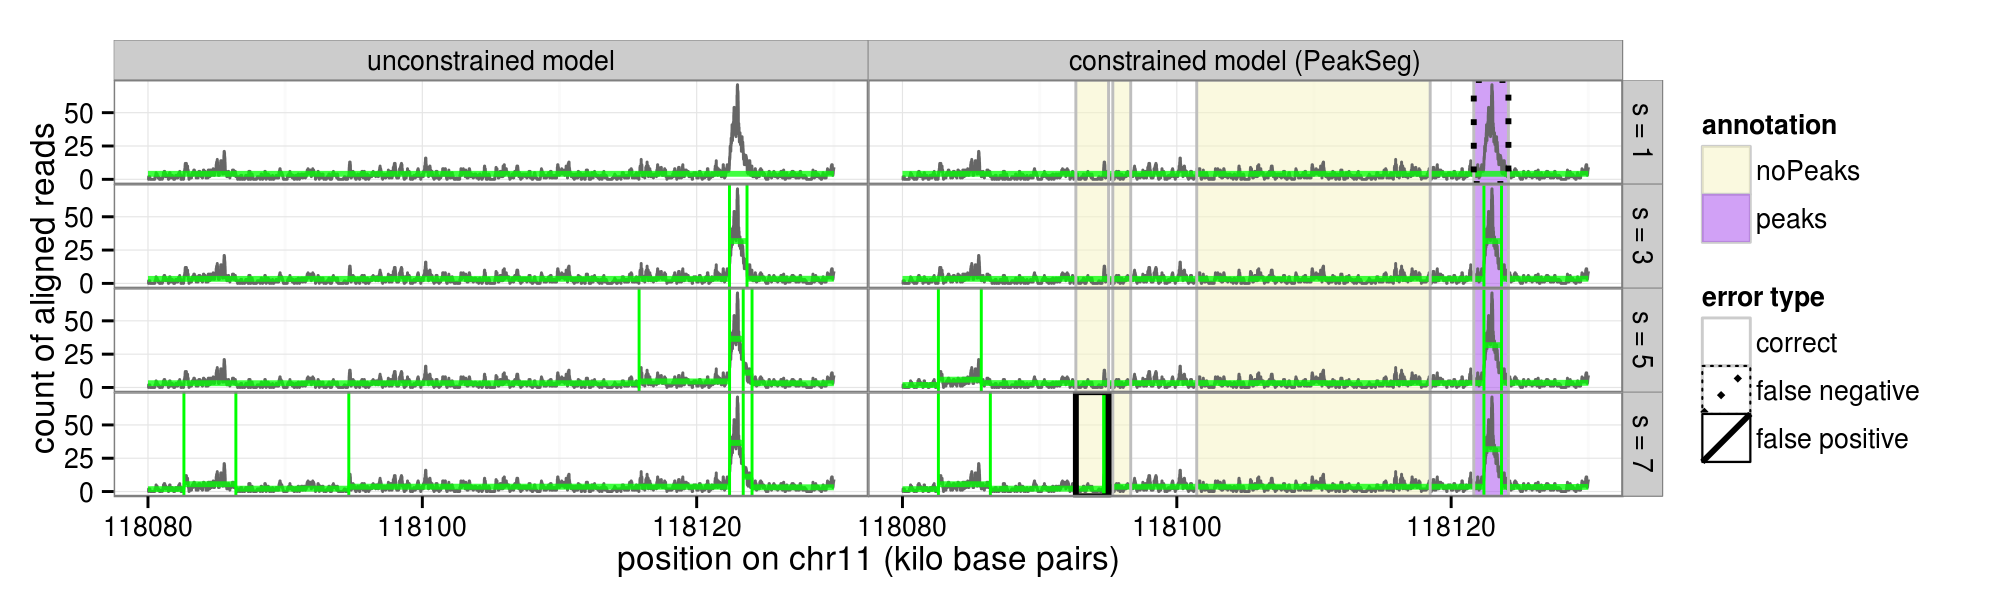
\includegraphics[width=\textwidth]{figure-Segmentor-PeakSeg}
  %\input{figure-Segmentor-PeakSeg}
  \vskip -0.5cm
  \caption{Example profile $\mathbf y$ (grey), with green horizontal
    lines for the segmentation mean $\mathbf m$, and green vertical
    lines to emphasize change-points. For this particular profile
    $\mathbf y$, the unconstrained and contrained models are
    equivalent $\mathbf{\hat m}^s(\mathbf y) = \mathbf{\tilde
      m}^s(\mathbf y)$ for $s\in\{1, 3\}$ segments but not for
    $s\in\{5, 7\}$. For the constrained models, the even-numbered
    segments are interpreted as peaks, whose accuracy can be
    quantified using the annotated region labels
    (\textcolor{peaks}{peaks} means there should be at least 1
    overlapping peak).}
  \label{fig:Segmentor-PeakSeg}
\end{figure*}

\subsection{Unsupervised ChIP-seq peak detectors}

There are literally dozens of unsupervised algorithms for peak
detection in ChIP-seq data sets, and the bioinformatics literature
contains several published comparison studies \citep{evaluation2010,
  rye2010manually, chip-seq-bench}. 

However, supervised peak detection model training is a relatively new
idea. \citet{hocking2014visual} proposed a benchmark of labeled
ChIP-seq data sets, with two different histone mark types: H3K4me3
(sharp peak pattern) and H3K36me3 (broad peak pattern). The best peak
detection algorithm in these H3K4me3 data was macs \citep{MACS}, and
the best for H3K36me3 was HMCan \citep{HMCan}. Both of these
algorithms are unsupervised, but were calibrated using the annotated
region labels to choose the best scalar significance threshold
hyperparameter via grid search.

\citet{DFilter} also attempted to train hyperparameters of
unsupervised peak detectors, and \citet{picking2012} found that
optimal values do not generalize between data sets. In contrast, we
show that our supervised \ref{PeakSeg} model can be trained for
accurate peak detection on test data that has the same type of peak
pattern.

\subsection{Maximum likelihood segmentation models}

The \ref{PeakSeg} model we propose in this paper is a constrained
version of the Poisson segmentation model of \citet{Segmentor}.
Their unconstrained model can be computed using a dynamic programming
algorithm (DPA) \citep{bellman}, or a pruned dynamic programming
algorithm (pDPA) \citep{pruned-dp}. Both algorithms are guaranteed to
recover the exact solution to the unconstrained model, but there are
two important differences. The pDPA is more complicated to implement,
but is also computationally faster than the DPA. For segmenting a
sequence of $d$ data points, the pDPA takes on average $O(d\log d)$
time whereas the DPA takes $O(d^2)$ time. 

Relative to the unconstrained segmentation model of \citet{Segmentor},
our proposed \ref{PeakSeg} model has an additional constraint. Rather
than searching all possible change-points to find the most likely
model with $s$ segments, we propose to constrain the possible
change-points to the subset of models that can be interpreted as peaks
(Section~\ref{sec:constrained}).

Due to the simplicity of its implementation, we propose a constrained
dynamic programming algorithm (cDPA) that requires a small
modification to the standard DPA solver. Although the DPA is an exact
solver for the unconstrained problem, we show that the cDPA is a
heuristic that is not guaranteed to solve the constrained
problem (Section~\ref{sec:dp-fails}). However, we show that it is
still very useful and accurate in practice on real data
(Section~\ref{sec:results}).

\subsection{Model selection criteria}

For each segmentation problem, the proposed cDPA returns a sequence of
models with $s\in\{1, 3, \dots, s_{\text{\text{max}}}\}$ segments. The
model selection problem is choosing a sample-specific number of
segments $s$ that maximizes the number of true positive peak
detections while minimizing the number of false positives. For
example, in Figure~\ref{fig:Segmentor-PeakSeg}, an ideal model
selection procedure would choose $s\in\{3, 5\}$ segments, since those
models have zero errors (\ref{eq:error}).

There are many unsupervised penalty functions for model selection. For
example, the classical AIC \citep{Akaike73} and BIC \citep{Schwarz78} are based
on theoretical asymptotic arguments. Several attempts have been made
to adapt the BIC for segmentation problems \citep{Yao88,
  mBIC}, and the non-asymptotic model selection theory of
\citet{cleynen2013segmentation} suggests another penalty function.

In the supervised setting of this paper, there is a training data set
of segmentation problems $i\in\{1, \dots, n\}$, with labeled regions
$R_i$ that can be used to compute the annotation error
(\ref{eq:error}). Thus, rather than taking a particular unsupervised
penalty function for granted, we can use the training data to learn
the penalty function with minimum error. In particular in
Section~\ref{sec:supervised-multi} we propose using the max margin interval
regression algorithm of \citet{HOCKING-penalties}, which was
originally proposed for learning a penalty function for optimal
change-point detection.

\section{From unconstrained to constrained maximum likelihoood
  segmentation}
\label{sec:model}

In this section we discuss Poisson maximum likelihood segmentation
models for count data. First, we discuss an existing unconstrained
model, and then we propose a constraint that makes the model suitable
for peak detection.

\subsection{Unconstrained maximum likelihood segmentation}

For a sequence of $d$ data points $\mathbf y\in\RR^d$ to segment, we
fix a maximum number of segments $1 \leq s_{\text{\text{max}}}\leq d$,
and define the unconstrained maximum likelihood segmentation problem
for any $s\in\{1, 2, \dots, s_{\max}\}$ as
\begin{align*}
  \label{unconstrained}
  \mathbf{\hat m}^s(\mathbf y)  =\ 
  &\argmin_{\mathbf m\in\RR^{d}} && 
  \rho
  \tag{\textbf{Unconstrained}}
  (\mathbf m, \mathbf y) \\
  &\text{such that} && \Segments(\mathbf m)=s,
\end{align*}
where the Poisson loss function is
\begin{equation}\label{eq:rho}
  \rho(\mathbf m, \mathbf y)= \sum_{j=1}^d m_j - y_j \log m_j.
\end{equation} 
The model complexity is the number of piecewise constant segments
\begin{equation}
  \Segments(\mathbf m)=1+\sum_{j=2}^d I(m_j \neq m_{j-1}),
\end{equation}
where $I$ is the indicator function. 

Although it is a non-convex optimization problem, the sequence of
segmentations $\mathbf{\hat m}^1(\mathbf y), \dots, \mathbf{\hat
  m}^{s_{\text{\text{max}}}}(\mathbf y)$ can be computed in
$O(s_{\text{\text{max}}} d^2)$ time using dynamic programming
\citep{bellman}, or in $O(s_{\text{\text{max}}} d \log d)$
time using pruned dynamic programming \citep{pruned-dp, Segmentor}.

This problem is ``\ref{unconstrained}'' in the sense that
$\mathbf{\hat m}^s(\mathbf y)$ is the most likely segmentation of all
possible models with $s$ piecewise constant segments ($s-1$
change-points). Several unconstrained models are shown on the left of
Figure~\ref{fig:Segmentor-PeakSeg}, and for example the second segment of the
model with $s=3$ segments appears to capture the peak in the data.
% In general, we would like to use the 2nd, 4th,
% ... segments as peaks, and the 1st, 3rd, ... segments as
% background. 
To construct a peak detector $c$, we first define the peak indicator at base
$j\in\{2, \dots, d\}$ as
\begin{equation}
  \label{eq:peaks}
  P_j(\mathbf m) = \sum_{k=2}^j \sign( m_{k} - m_{k-1} ),
\end{equation}
where $P_1(\mathbf m)=0$ by convention. $P_j(\mathbf m)$ is the
cumulative sum of signs of changes up to point $j$ in the piecewise
constant vector $\mathbf m$. We define the vector of peak indicators
as
\begin{equation}
  \mathbf
P[\mathbf m] = \left[\begin{array}{ccc} P_1(\mathbf m) & \cdots &
    P_d(\mathbf m)
\end{array}\right].
\end{equation}

\subsection{PeakSeg: constrained maximum likelihood}
\label{sec:constrained}

In general for the unconstrained model $P_j(\mathbf m)\in\ZZ$, which
is problematic since we want to use it as a peak detector with binary
outputs $P_j(\mathbf m)\in \{0, 1\}$. 

For example, if $\mathbf m = \left[\begin{array}{ccccccc}1.1 &
    1.1 & 2 & 2 & 4 & 4 & 3\end{array}\right]$, with two changes up
followed by one change down, then $\mathbf P(\mathbf m) =
\left[\begin{array}{ccccccc}0 & 0 & 1 & 1 & 2 & 2 &
    1 \end{array}\right]$.

% This is also a practical problem that can be observed in real data
% sets. For example in Figure~\ref{fig:Segmentor-PeakSeg} there is a position $j$ for
% which $P_j\left[ \mathbf{\hat m}^5(\mathbf y) \right]=2$ (since the
% mean changes up, up, down, down). 

Thus we constrain the peak indicator $P_j(\mathbf
m)\in\{0, 1\}$, which results
in the constrained problem
\begin{align*}
  \label{PeakSeg}
  \mathbf{\tilde m}^s(\mathbf y)  =
    \argmin_{\mathbf m\in\RR^{d}} &\ \ 
    \rho(\mathbf m, \mathbf y) 
    \tag{\textbf{PeakSeg}}
\\
    \text{such that} &\ \  \Segments(\mathbf m)=s,  \\
     \forall j\in\{1, \dots, d\}, &\ \ P_j(\mathbf m) \in\{0, 1\}.
\end{align*}
Note that one must specify the number of segments $s$ or,
equivalently, the number of peaks $p=(s-1)/2$. Another way to
interpret the constrained \ref{PeakSeg} problem is that the sequence
of changes in the segment means $\mathbf m$ must begin with a positive
change and then alternate: up, down, up, down, ... (and not up, up,
down). Thus the even-numbered segments may be interpreted as peaks
$P_j(\mathbf m)=1$, and the odd-numbered segments may be interpreted
as background $P_j(\mathbf m)=0$.

For example, the good peaks in Figure~\ref{fig:dp-peaks-train} are the
the second and fourth segments of the \ref{PeakSeg} solution for $s=5$
segments.

Figure~\ref{fig:Segmentor-PeakSeg} shows a profile where the constraint is
necessary for the even-numbered segments to be interpreted as
peaks. In particular, it is clear that unconstrained models with
$s\in\{5, 7\}$ segments do not satisfy $P_j[\mathbf{\hat m}^s(\mathbf
y)]\in\{0, 1\}$ for all positions $j\in\{1,\dots, d\}$ (since they
have up, up, down changes).

\section{Algorithms}
\label{sec:algorithms}

In this section we first review the existing standard dynamic
programming algorithm (DPA) for segmentation, then propose a new
constrained dynamic programming algorithm (cDPA). We also give a
counter-example which shows that the cDPA is a heuristic for solving
the \ref{PeakSeg} optimization problem.

\subsection{The standard DPA}

The \ref{unconstrained} model can be computed exactly using a dynamic
programming algorithm (DPA).
% To describe this algorithm we
% define $\widehat{\mathcal{L}}_{s,t}$ as minus the best log-likelihood of
% the segmentation $\widehat{m}_{s,t}$.  This best log-likelihood can be
% written as the sum of the best log-likelihood of its segment.  
Let $t,t'$ be indices such that $0\leq t' < t \leq d$, and let the
interval $(t', t]$ denote a segment. Then $\sigma_{(t', t]} =
\sum_{j=t'+1}^t y_j$ is the cumulative sum and $M_{(t', t]} =
\sigma_{(t', t]}/(t-t')$ is the mean over the segment $(t', t]$. The
optimal Poisson loss (\ref{eq:rho}) for that segment is
\begin{equation}
  \label{eq:log-lik-segment}
  c_{(t',t]} = \sigma_{(t', t]}\left[1 - 
  \log\left(M_{(t', t]}\right)\right].
\end{equation}
Let ${\mathcal L}_{s, t}$ be the optimal Poisson loss of the
model with $s$ segments up to data point $t$ and ${\mathcal T}_{s, t}$ the corresponding optimal last change. The key idea behind the
DPA is that 
if we consider an optimal segmentation in $s$ up to $t$ and consider
the subsegmentation obtained by discarding the last segment $({\mathcal T}_{s, t}, t]$ then
the resulting segmentation is also optimal in the sense that its loss is equal to ${\mathcal L}_{s-1, {\mathcal T}_{s, t}}.$
%any subsegmentation of an optimal segmentation
%should be optimal. 
This can be formally written as a search for the best
change-point $t'$
\begin{equation}
{\mathcal{L}}_{s,t}= \min_{t' < t}
{\mathcal{L}}_{s-1,t'} +
 c_{(t',t]}, 
 \label{eq:update1}
\end{equation}
meaning that the best loss in $s$ segments can be written in terms of
the best loss in $s-1$ segments. Using this update
rule iteratively for all $s$ from $2$ to $s_{\text{max}}$ and for all
$t$ from $2$ to $d$ we recover the best segmentations in $1$ to
$s_{\text{max}}$ in $\mathcal{O}(s_{\text{max}}d^2)$ time.

%\begin{algorithm}[H]
%\begin{algorithmic}[1]
%\FOR{$d=2$ to $D_{\text{max}}$}
%\FOR{$\tau'=d$ to $n$}
%\STATE $ \mathbf{L}_{d,\tau'+1} = \min_{\tau \leq \tau'} \{ \ \mathbf{L}_{d-1,\tau} + C_{\tau, \tau'+1} \ \}$
%\STATE $ \mathbf{m}_{d,\tau'+1} = \arg \min_{\tau \leq \tau'} \{ \ \mathbf{L}_{d-1,\tau} + C_{\tau, \tau'+1} \ \}$
%\ENDFOR
%\ENDFOR
%\caption{Dynamic Programming for Poisson segmentation model}
%\end{algorithmic}\label{algo:v1}
%\end{algorithm}

\subsection{cDPA: a simple modification}
\label{sec:constrained-dp}

In order to force the segmentation to obey the constraints of the
\ref{PeakSeg} model, we introduce a simple modification of the
previous update rule (\ref{eq:update1}). %algorithm %\ref{algo:v1}.
Up to now we considered all possible change-points $t'$ smaller than
the current $t$. Here we propose to consider only those such that the
resulting segmentation can be interpreted as a succession of
peaks. To make this idea more precise we introduce the notation
$\mathcal{E}_{s,t}$ which is the last empirical mean of the best
segmentation in $s$ segments up to $t$.  

Then if $s$ is even (peak segment) the mean of segment $(t', t]$
should be larger than the previous one and in the update rule we only
consider $t'$ such that
\begin{equation}
  \label{eq:even}
   t' < t \ | \ \mathcal{E}_{s-1,t'} < M_{(t', t]}.
\end{equation}
On the contrary, if $s$ is odd (background segment) the mean of
segment $(t', t]$ should be smaller than the previous one and we
consider only $t'$ such that
\begin{equation}
  \label{eq:odd}
   t' < t \ | \ \mathcal{E}_{s-1,t'} > M_{(t', t]}.
\end{equation}
In the end we get the following algorithm:\footnote{Implemented as C
  code in the R package\\ \url{https://github.com/tdhock/PeakSegDP}}
\newcommand{\SWITCH}[1]{\STATE \textbf{switch} (#1)\begin{ALC@g}}
\newcommand{\ENDSWITCH}{\end{ALC@g}\STATE \textbf{end switch}}
\newcommand{\CASE}[2]{\STATE \textbf{case} #1\textbf{: } #2}%\begin{ALC@g}}
\newcommand{\ENDCASE}{}%\end{ALC@g}}
\newcommand{\DEFAULT}[1]{\STATE \textbf{default: } \begin{ALC@g}}
\newcommand{\ENDDEFAULT}{\end{ALC@g}\STATE \textbf{end default} }
\newcommand{\FORFOR}[2]{\STATE \textbf{For} #1 \textbf{do} and \textbf{For} #2 \textbf{do} \begin{ALC@g}}
\newcommand{\ENDFORFOR}{\end{ALC@g}\STATE \textbf{End for} and \textbf{End for}  }

\begin{algorithm}[H]
\begin{algorithmic}[1]
\REQUIRE $\mathbf y\in\RR^d$, $s_{\text{max}}\in\{2, \dots, d\}$.
%\STATE \textbf{TODO:} initialize ${\mathcal L}_1, t$ ?
\FORFOR{($s=2$ to $s_{\text{max}}$)}{($t=s$ to $d$)}
\SWITCH{$s$}
\CASE{even}{$T \gets \{ t' < t \mid \mathcal{E}_{s-1,t'} < M_{(t', t]} \}$}
\ENDCASE
\CASE{ odd}{$T \gets \{ t' < t \mid \mathcal{E}_{s-1,t'} > M_{(t', t]} \}$}
\ENDCASE
\ENDSWITCH

\SWITCH{$T$}
\CASE{$\emptyset$}{${ \mathcal L}_{s,t} \gets \infty$}
\ENDCASE
\DEFAULT{}
\STATE $ \mathcal T_{s, t}\gets t^* \gets
\underset{ t'\in T}{\arg \min}\  {\mathcal{L}}_{s-1,t'} + c_{(t',t]}$
\STATE $ {\mathcal{L}}_{s,t} \gets 
{\mathcal{L}}_{s-1,t^*} + c_{(t^*,t]} $
\STATE $\mathcal{E}_{s,t} \gets M_{(t^*, t]}$
\ENDDEFAULT
\ENDSWITCH
\ENDFORFOR
\RETURN $s_{\text{max}}\times d$ matrix $\mathcal T_{s, t}$ of optimal change points.
\caption{Constrained dynamic programming (cDPA) 
%for Poisson  segmentation model
}
\end{algorithmic}\label{algo:v2}
\end{algorithm}

Note that we do not need to precompute the $d(d-1)/2$ values of
$c_{(t',t]}$ and $M_{(t', t]}$. That is because the optimal cost
$c_{(t',t]}$ and empirical mean $M_{(t', t]}$ are simple functions of
$\sigma_{(t', t]} =\sum_{j=t'+1}^t y_j$ which can be computed in
$\mathcal{O}(1)$ given the cumulative sum of the data-points,
$\sum_{j=1}^t y_j$. Hence the computational requirements of the cDPA
are the same as the DPA: $\mathcal{O}(s_{\text{max}} d)$ memory and
$\mathcal O(s_{\text{max}} d^2)$ time.

Note also that for both the even and odd update it might very well be
that the set of possible changes $T$ is empty.  This means that no
segmentation in $s$ segments to point $t$ satistifying the
\ref{PeakSeg} model constraint was found.  To cope with this case we
simply set ${\mathcal L}_{s, t} = \infty$.

Hence the cDPA is not guaranteed to recover a segmentation. In
particular for an ever increasing series of data $y_1 < \cdots < y_d$,
for example $\mathbf y = \left[ \begin{array}{ccc} 1 & 2 &
    3 \end{array}\right]$ the constrained optimal segmentation
$\mathbf{\tilde m}^3(\mathbf y)$ is undefined, and the cDPA thus
returns no model.
% Indeed in that case for any segmentation the empirical mean of
% the third segment is necesarily larger than the empiricial mean of the
% second segment (which is in contradiction with our constraint).

\subsection{The cDPA is a heuristic}
\label{sec:dp-fails}

In this section we give a simple counter-example which shows that the
cDPA is not guaranteed to recover a valid \ref{PeakSeg} model even if
there is one.  This is mostly a theoretical issue, since 
the cDPA is empirically able to compute \ref{PeakSeg} models in the vast
majority of real data sets
(Section~\ref{sec:heuristic-effectiveness}).

The cDPA is a heuristic in the sense that it is not clear which
optimization problem it solves. In particular, it does not necessarily
recover the maximum likelihood segmentation that satistifies the
\ref{PeakSeg} model constraints. We illustrate this using the following simple
example with $\mathbf y = \left[\begin{array}{cccc} 1 & 10 & 14 & 13
\end{array}\right]\in\ZZ_+^4
$. For $s=3$ segments there are only 3 possible segmentations:
$[1][10][14, 13]$, $[1][10, 14][13]$ and $[1, 10][14][13]$. If we use
max-likelihood estimates for each segment mean, then only the last
segmentation obeys the \ref{PeakSeg} model constraints. However the
cDPA will not recover it.

That is because the best segmentation recovered by the cDPA for $s=2$
segments up to point $3$ is $[1][10, 14]$.
% Its likelihood
% is $(1 + 0) + (10+14 + (10+14)\log(24/2)) \approx 84.6 $ which is
% indeed larger than the likelihood of $[1, 10][14]$: $(11 +
% 11\log(11/2)) + (14\log(14)) \approx 66.69 $. 
For $s=3$ the cDPA will then consider the segmentations $[1][10][14,
13]$ and $[1][10, 14][13]$ and discard them since they do not satisfy
the \ref{PeakSeg} model constraints. The cDPA will thus report that it
didn't find a valid peak model in $s=3$. However there is one: $[1,
10][14][13]$.

Note that if we run the constrained DP in the backward direction, 
$\mathbf y = \left[\begin{array}{cccc} 13 & 14 & 10 & 1
\end{array}\right]\in\ZZ_+^4
$, we would recover the best solution $[13][14][10, 1]$.


% \subsection{Constrained dynamic programming}
% \label{sec:constrained-dp}

% We propose to use dynamic programming to compute the sequence of
% maximum likelihood models $\mathbf{\tilde m}^1(\mathbf y), \dots,
% \mathbf{\tilde m}^{s_{\text{\text{max}}}}(\mathbf y)$ satisfying this up-down
% constraint.

% \textbf{TODO}: more detailed description of dynamic programming.

% The algorithm is in $O(s_{\text{\text{max}}} d^2)$ time, where $d$ is the
% number of data points, using the compression scheme proposed by
% \citet{Segmentor}. A free/open-source R package implementing the
% dynamic
% programming is available at\\
% \url{https://github.com/tdhock/PeakSegDP}

% \subsection{Constrained DP is a heuristic}
% \label{sec:dp-fails}
% \textbf{TODO}: discussion of when the DP does not recover the optimal
% solution. Maybe a figure? Maybe not. Maybe a discussion of how many
% times it returned all 10 models in the real data sets.

\section{Penalty function learning methods}
\label{sec:penalty-learning}

For a profile $\mathbf y\in\RR^d$ and a penalty constant $\lambda\in\RR_+$, the
optimal number of segments is
\begin{equation}
  \label{eq:optimal_segments}
  s^*(\lambda, \mathbf y) =
  \argmin_{s\in\{1,3,\dots, s_{\text{\text{max}}}\}}
  \rho\left[
    \mathbf{\tilde m}^s(\mathbf y),
    \mathbf y
  \right]
  + h(s, d) \lambda,
\end{equation}
where $h(s, d)$ is a model complexity function that is given. In
this paper we consider two types of model complexity $h$ functions:
AIC/BIC and oracle (Table~\ref{tab:penalties}). 

For each training sample $i\in\{1,\dots, n\}$, we have a feature
vector $\mathbf x_i\in\RR^m$ (details in
Section~\ref{sec:supervised-multi}). We learn a penalty function
$f(\mathbf x_i) = \log \lambda_i$ that predicts a sample-specific
number of segments $s^*(\lambda_i, \mathbf y_i)$ with minimum train
error.

After learning a penalty function $\hat f$ on the training
data, we use the following method to make a prediction on a test
sample with profile $\mathbf y$ and features $\mathbf x$. We compute
the predicted penalty $\hat \lambda = \exp \hat f(\mathbf x)$, the
predicted number of segments $\hat s = s^*(\hat \lambda, \mathbf y)$,
and the predicted peaks $\mathbf P\left[ \mathbf{\tilde
    m}^{\hat s}(\mathbf y) \right]$.

\subsection{Unsupervised penalty learning}
\label{sec:unsupervised}

% After computing the constrained maximum likelihood segmentations for
% each sample $i\in\{1,\dots, n\}$, the only question that remains is:
% how many segments?

There are several unsupervised penalty functions that are based on theoretical
assumptions about the data (distribution, independence) which may or
may not be true in practice. One can use asymptotic arguments to get a
penalty such as the AIC \citep{Akaike73}, BIC \citep{Schwarz78}, or
mBIC \citep{mBIC}. For example, the AIC corresponds to a constant
penalty of $\lambda=\exp f(\mathbf x)=2$ and a model complexity of
$h(s, d)=s$. More recently, \citet{cleynen2013segmentation} applied
finite sample model selection theory to obtain a more complicated
model complexity function $h$ (Table~\ref{tab:penalties}) and a
heuristic for computing the penalty $\lambda$. All of these penalty
functions are completely unsupervised since they ignore the annotated
region labels in the training data set.

In Table~\ref{tab:penalties} and Figure~\ref{fig:test-error}, these
models are named *.0 since they do not learn any parameters using the
training data.

\subsection{Supervised single-parameter penalty learning}
\label{sec:supervised-single}

\citet{cleynen2013segmentation} proposed to use the un\-supervised
heuristic of \citet{arlot2009data} for calibrating the penalty constant
$\beta$ in equation (6) of their paper. Instead, we propose to use the
annotated region labels as a super\-vised method for calibrating the
penalty constant $\beta$. This corresponds to learning a constant
penalty function $\exp f(\mathbf x_i) = \beta = \lambda_i$ for all
samples $i$.

More specifically, we defined a grid of 200 $\beta$ penalty constants
evenly spaced on the log scale between $10^{-2}$ and $10^4$, then used
grid search to select the value that minimizes the annotation error
(\ref{eq:error}) on the train set.

In Table~\ref{tab:penalties} and Figure~\ref{fig:test-error}, these
models are named *.1 since they each learn 1 parameter using the
training data.

\subsection{Supervised multi-parameter penalty learning}
\label{sec:supervised-multi}

For supervised learning of multi-parameter penalties, we
define sample-specific penalty values $\log \lambda_i = f(\mathbf
x_i)= \beta + \mathbf w^\intercal \mathbf x_i$, which is an affine
function with parameters $\beta\in\RR,\mathbf w\in\RR^m$ that will be
learned. As shown in Table~\ref{tab:penalties}, we considered learning
models with 3 and 41 parameters:

\begin{itemize}
\item \textbf{3}: we used an $m=2$-dimensional feature
  vector $\mathbf x_i = \left[\begin{array}{cc} \log\max \mathbf y_i &
      \log d_i
\end{array}\right]$ where $\mathbf y_i\in\RR^{d_i}$ 
is one sample $i$ of count data to segment.
This corresponds to a penalty $\lambda_i = e^\beta (\max\mathbf
y_i)^{w_1} d_i^{w_2}$. We fit the model by solving the un-regularized
interval regression problem of \citet{HOCKING-penalties}.
\item \textbf{41}: we defined $m=40$ features using transforms ($x,
  \log x, \log[x+1], \log\log x$), where $x$ are features such as
  quartiles of $\mathbf y_i$, mean of $\mathbf y_i$, and
  number of data points $d_i$. We fit the model by solving
  the L1-regularized problem of
  \citet{HOCKING-penalties}.
\end{itemize}


\begin{table*}[b!]

  \begin{minipage}{0.4\textwidth}
  \begin{tabular}{ll}
    \textbf{name} & \textbf{model complexity} $h(s, d_i)$ \\
    \hline
    AIC/BIC.* & $s$\\
    oracle.* & $s\left(1 + 4\sqrt{1.1 + \log(d_i/s)}\right)^2$
  \end{tabular}
  \end{minipage}
  \begin{minipage}{0.5\textwidth}
  \begin{tabular}{lllll}
    \textbf{name} & \textbf{smoothing} $\lambda_i$ & 
    \textbf{parameters} & \textbf{learning algorithm} \\
    \hline
    *.0 & AIC=2, BIC=$\log d_i$ & none & unsupervised \\
    *.1 & 
    $\beta$ & 
    $\beta\in\RR_+$ & grid search \\
    *.3 & 
    $e^\beta d_i^{w_1} (\max \mathbf y_i)^{w_{2}}$ & 
    $\beta, w_1, w_{2}\in\RR$ & interval regression \\
    *.41 & 
    $\exp(\beta + \mathbf w^\intercal \mathbf x_i)$ & 
    $\beta\in\RR, \mathbf w\in\RR^{40}$ & 
    regularized int. reg. \\
  \end{tabular}
  \end{minipage}

  \caption{Penalties for model selection (\ref{eq:optimal_segments}) 
    are of the form
    $h(s, d_i) \lambda_i $ 
    for data to segment $\mathbf y_i\in\RR^{d_i}$ 
    and models with $s$ segments. 
    Names show model complexity
    $h(s, d_i)$ (left) and number of parameters to learn in $\lambda_i$ (right).
    For example, the AIC/BIC.41 model has a penalty of
    $s \exp(\beta + \mathbf w^\intercal \mathbf x_i)$, 
    where the parameters $\beta,\mathbf w$ 
    are learned using regularized interval regression 
    on a training data set.
  }
  \label{tab:penalties}
\end{table*}

\begin{figure*}[b!]
  \centering
  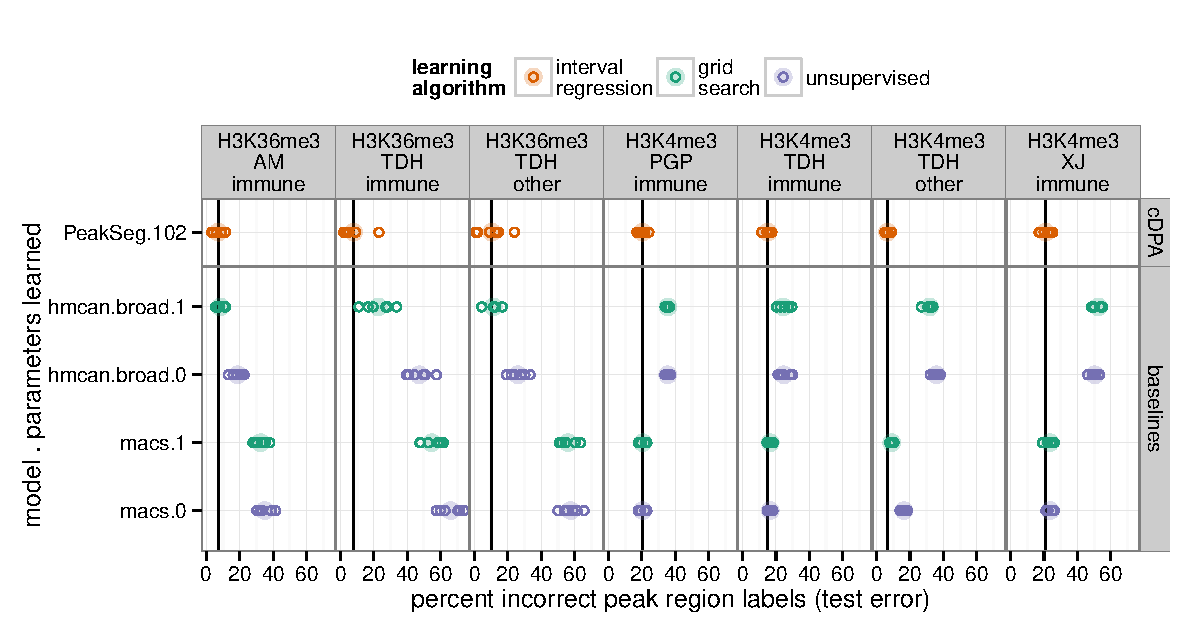
\includegraphics[width=\textwidth]{figure-dp-peaks-regression-dots}
  \vskip -0.5cm
  \caption{Test error of peak detection algorithms on seven labeled
    data sets (each point shows one of six randomly selected
    train/test splits, the shaded circle is the mean test error, and
    the vertical black line is the mean of the best algorithm for each
    data set). Data set names show data/pattern type (e.g. H3K36me3),
    annotator (AM), and cell types (immune). Colors show how the
    training data were used to learn model parameters.}
  \label{fig:test-error}
\end{figure*}

\section{Results: state-of-the-art peak detection
  for two patterns}
\label{sec:results}

We downloaded 7 benchmark data sets, which included a total of 12,826
manually annotated regions across 2,752 separate segmentation
problems.\footnote{\url{http://cbio.ensmp.fr/~thocking/chip-seq-chunk-db/}}
Data sets span two different data/pattern types (sharp H3K4me3, broad
H3K36me3), four annotators (AM, TDH, PGP, XJ), and two cell type
groups (immune, other). Each data set contains labels grouped into
windows of nearby regions (from 4 to 30 windows per data set). For
each data set, we performed 6 random splits of windows into half
train, half test.  We
considered 3 kinds of model training:\footnote{Source code for computing models and benchmarks at\\
  \url{https://github.com/tdhock/PeakSeg-paper} }
\begin{itemize}
\item \textbf{Unsupervised} uses the default parameters of each
  algorithm, ignoring the labeled data in the train set.
\item \textbf{Grid search} learns a scalar parameter with minimal
  annotation error on the train set.
\item \textbf{Interval regression} is the multi-parameter
  penalty learning model of \citet{HOCKING-penalties}.
\end{itemize}

\subsection{Effectiveness of heuristic cDPA}
\label{sec:heuristic-effectiveness}

To run the cDPA on the benchmark data set, we first set the maximum
number of segments $s_{\text{\text{max}}}=19$, meaning a maximum of $9$
peaks. 
% Running the cDPA on all of the data sets in the benchmark took
% a total of about 6.5 days. For the largest profile we considered
% ($d=263,169$ data points), the cDPA took
% about 155 minutes. 
As discussed in Section~\ref{sec:dp-fails}, the cDPA is a heuristic
for computing the \ref{PeakSeg} model. To assess whether or not this
is a problem in real data sets, we checked for how many segmentation
problems the cDPA returned the complete sequence of 10 models
$\mathbf{\tilde m}^1(\mathbf y),\mathbf{\tilde m}^3(\mathbf y), \dots,
\mathbf{\tilde m}^{19}(\mathbf y)$. For the vast majority of
segmentation problems ($2738/2752=99.5\%$), the constrained DP returned
all 10 models. For the other 14 problems, the algorithm did not return
at least one of the ten models. Of these 14 problems with missing
models, 11 problems still had at least one perfect peak detection
model with zero annotation error~(\ref{eq:error}). We concluded that
although the cDPA is technically a heuristic algorithm for
solving \ref{PeakSeg}, it is still a useful peak detector in the vast
majority of real data sets.

% \subsection{Baseline peak detection algorithms}

% We compared the proposed PeakSeg algorithm to the two previous
% state-of-the-art peak detectors on this benchmark, macs and
% \mbox{hmcan.broad}. 

\subsection{Comparison of unsupervised methods}

In a previous study of this benchmark data set
\citep{hocking2014visual}, the macs algorithm was found to be the most
accurate peak detector for H3K4me3 data, whereas hmcan.broad was best
for H3K36me3 data.

Figure~\ref{fig:test-error} shows that in three H3K36me3 data sets
(broad peak pattern), hmcan.broad.0 is clearly more accurate than
macs.0. Furthermore, it is clear that the oracle.0 model is at least
as accurate as hmcan.broad.0.

For the four H3K4me3 data sets (sharp peak pattern), oracle.0 is about
as accurate as macs.0, which is clearly more accurate than
hmcan.broad.0.

Finally, the unsupervised AIC/BIC.0 method is clearly the least
accurate of all methods, since it always picks the model with the most
peaks (same as no penalty). We also tried the modified BIC of
\citet{mBIC}, but obtained the same high false positive rates.

\subsection{Supervised learning of 1 parameter increases peak
  detection accuracy}

Does training a single scalar parameter using grid search increase
peak detection accuracy relative to unsupervised default models? Yes,
in the vast majority of cases. Figure~\ref{fig:test-error} shows that
supervised *.1 models have generally lower test error than the
corresponding unsupervised *.0 models.

Among models with only 1 parameter trained using grid search, it is
clear that oracle.1 is the most accurate. It achieves close to
state-of-the-art peak detection accuracy on every data set. In
contrast, the baseline macs.1 is only effective for H3K4me3 data, and
the baseline hmcan.broad.1 is only effective for H3K36me3 data.

\subsection{Supervised learning of several parameters can further
  increase peak detection accuracy}

Does supervised multi-parameter model training improve over
single-parameter models? A little, if there are sufficient training
data. Figure~\ref{fig:test-error} shows that multi-parameter models
(*.3 and *.41) tend to be at least as accurate as the corresponding
single-parameter *.1 model. The only exceptions are the H3K36me3\_TDH
data sets, for which there are few training data (only 2 groups of
labeled regions per train set). For these data, the *.3 and
*.41 models sometimes overfit relative to the corresponding *.1 model.

\section{Discussion}
\label{sec:discussion}

\subsection{Supervised versus unsupervised learning}

Baseline unsupervised peak detectors in the bioinformatics literature
are each designed to recognize a specific peak pattern. For example we
observed that the macs algorithm was effective for the sharp peak
pattern in H3K4me3 data, and the hmcan.broad algorithm was effective
for the broad peak pattern in H3K36me3.

In contrast, we propose a supervised learning approach for peak
detection. Rather than designing a specific model for each pattern, we
propose to use a database of labels with a general peak detector that
can be trained to recognize different patterns. We showed that
supervised penalty learning with the \ref{PeakSeg} model can be used
for accurate peak detection in both H3K4me3 and H3K36me3 data.

In general, it is clear that the supervised learning methods were more
accurate than their unsupervised counterparts. The only exception is
that sometimes when there are few training data, the multi-parameter
supervised learning methods overfit (Figure~\ref{fig:test-error},
H3K36me\_TDH data sets). So when there are very few training data, we
recommend using the oracle.1 supervised model which avoids overfitting
by learning just 1 parameter using grid search. However, when there
are many training data, we would recommend using a multi-parameter
supervised learning method such as oracle.41.

\subsection{Oracle penalty is more accurate than AIC/BIC}

We tested the peak detection accuracy of two types of model complexity
$h$ functions (Table~\ref{tab:penalties}). Among unsupervised models,
Figure~\ref{fig:test-error} shows that the oracle.0 model is always
more accurate than the AIC/BIC.0 model. For the supervised 1-parameter
models, it is also clear that oracle.1 is more accurate than
AIC/BIC.1. However, we obtained similar test error rates when we used
multi-parameter supervised learning with AIC/BIC and oracle
penalties.

In general, these data provide convincing evidence that the model
selection theory of \citet{cleynen2013segmentation} is useful for
accurate peak detection in real ChIP-seq data sets, especially when
combined with supervised penalty learning methods.

% \begin{figure*}[t!]
%   \centering
%   \includegraphics[width=\textwidth]{figure-regularized-all}
%   \vskip -0.5cm
%   \caption{Normalized weights of the 2-feature log.bases.log.max model
%     compared to the 41-feature L1.reg model. In some data sets the
%     L1.reg model sets these feature weights to 0.}
%   \label{fig:regularized-all}
% \end{figure*}

% \begin{figure*}[t!]
%   \centering
%   \includegraphics[width=\textwidth]{figure-regularized-feature-importance}
%   \vskip -0.5cm
%   \caption{Importance of features in L1.reg models. There were several
%     features in H3K4me3 data sets which were selected in all 6
%     train/test splits (note that unweighted.quartile.100\% is the same
%     as the maximum of the data). For other data sets it is not clear
%     which features are most important.}
%   \label{fig:regularized-feature-importance}
% \end{figure*}

\section{Conclusions and future work}
\label{sec:conclusions}

We proposed the \ref{PeakSeg} constrained maximum likelihood
segmentation model as a peak detector in ChIP-seq count data. We
proposed a constrained dynamic programming algorithm that efficiently
computes a sequence of segmentations that satisfy the \ref{PeakSeg}
constraint. Furthermore, we proposed to use annotated region labels as
supervision in a penalty learning problem. Whereas unsupervised
baseline methods are only effective for a single data/pattern type, our
approach yields state-of-the-art peak detection in a benchmark that
includes both sharp H3K4me3 and broad H3K36me3 data/pattern types.

There are several modeling choices that could be explored to increase
peak detection accuracy. First, we could replace the Poisson
assumption of the \ref{PeakSeg} model with a negative binomial
distribution \citep{cleynen2013segmentation}, which has an additional
variance parameter. Also, a more accurate model could possibly be
obtained by engineering better features $\mathbf x_i$, and learning a
non-linear smoothing function $f$. Finally, one could imagine 
learning model complexity functions $h$. For example the oracle
penalty of \citet{cleynen2013segmentation} has an assumed constant of
1.1 (Table~\ref{tab:penalties}), which could be learned instead.

The current implementation of \ref{PeakSeg} using the cDPA has several
limitations. First, the $O(d^2)$ time complexity for $d$ data points
could be easily reduced to $O(d\log d)$ by using a constrained version
of pruned dynamic programming \citep{pruned-dp, Segmentor}. Second, we
showed that the cDPA is a heuristic for computing the \ref{PeakSeg}
model (Section~\ref{sec:dp-fails}). On one hand, we would like to know
what optimization problem the cDPA solves. On the other hand, we would
like an efficient algorithm that exactly computes the \ref{PeakSeg}
model.

Finally, we are interested in segmenting multiple samples $i$ at the
same time, since peaks are often observed in the same genomic location
across several samples of the same cell type. This joint peak
detection problem may lead to more accurate peak calls, but it is a
considerably more difficult segmentation problem.

% \begin{table*}[b!]
%   \centering
%   \begin{tabular}{ccc}
%     \textbf{learning algorithm} & \textbf{heuristics} & 
%     \textbf{constrained optimization} \\
%     \hline
%     unsupervised & hmcan.broad.0, macs.0 & AIC/BIC.0, oracle.0 \\
%     grid search & hmcan.broad.1, macs.1 & AIC/BIC.1, oracle.1 \\
%     interval regression & --- & AIC/BIC.3, oracle.3 \\
%     regularized interval regression & --- & AIC/BIC.41, oracle.41 \\
%   \end{tabular}
%   \caption{Comparison of peak detection methods for ChIP-seq data. 
%     The two main contributions of this paper 
%     are to show that peak detection can be improved 
%     using constrained optimization and 
%     interval regression to learn a 
%     multi-parameter penalty function.}
%   \label{tab:supervised-maxlik}
% \end{table*}

\newpage


\bibliographystyle{abbrvnat}

\bibliography{refs}

\end{document}
